\documentclass[12pt]{article}
\usepackage{../../template}
\author{niceguy}
\title{Lecture 7}
\begin{document}
\maketitle

\section{Taylor Series and Approximations for Two-Variable Functions}

A first approximation for a function at somewhere near $x_0$ can simply be
$$f(x_0+\Delta x) \approx f(x_0)$$
To make this a better approximation, we could consider the \textit{tangent} at $x_0$, which gives us the slightly more "accurate" approximation
$$f(x_0+\Delta x) = f(x_0) + f'(x_0)\Delta x$$A first approximation for a function at somewhere near $x_0$ can simply be
$$f(x_0+\Delta x) \approx f(x_0)$$
To make this a better approximation, we could consider the \textit{tangent} at $x_0$, which gives us the slightly more "accurate" approximation
$$f(x_0+\Delta x) = f(x_0) + f'(x_0)\Delta x$$
We can then have a quadratic approximation
$$f(x_0+\Delta x) = f(x_0) + f'(x_0)\Delta x + \frac{1}{2}f''(x_0)\Delta x^2$$
and so on. In general, the n$^{\text{th}}$ degree taylor polynomial is given by
$$f(x_0+\Delta x) = \sum_{i=1}^n \frac{1}{i!}f^{(n)}(x_0) \Delta x^n$$
Let us consider the two dimensional case. Let $P$ be the known point, and $Q$ be the point we wish to approximate. Then the parametric equations of line $PQ$ is
\begin{align*}
	x(t) &= x_0 + \Delta x t \\
	y(t) &= y_0 + \Delta y t
\end{align*}
where $t \in [0,1]$. \\
We then define
$$F(t) = f(x_0+\Delta x, y_0+\Delta y)$$
We now have a single variable function $F(t)$. Note that $F(0) = f(x_0,y_0)$ and $F(1) = f(x_0+\Delta x, y_0+\Delta y)$. We want to estimate $F(1)$.

$$F'(t) = \frac{d}{dt}F(t) = \frac{\partial f}{\partial x} \frac{dx}{dt} + \frac{\partial f}{\partial y} \frac{dy}{dt} = \frac{\partial f}{\partial x} \Delta x + \frac{\partial f}{\partial y}\Delta y$$
The second derivative is then
$$F''(t) = \frac{d}{dt}\left(\frac{\partial f}{\partial x}\Delta x + \frac{\partial f}{\partial y} \Delta y\right) = \frac{\partial^2 f}{\partial x^2} \frac{dx}{dt} \Delta x + \frac{\partial^2 f}{\partial y \partial x} \frac{dy}{dt} \Delta x + \frac{\partial^2 f}{\partial x \partial y} \frac{dx}{dt} \Delta y + \frac{\partial^2 f}{\partial y^2} \frac{dy}{dt} \Delta y$$
If Clairaut's Theorem holds,
$$F''(t) = \frac{\partial^2 f}{\partial x^2} \Delta x^2 + 2\frac{\partial^2 f}{\partial x \partial y} \Delta x \Delta y + \frac{\partial^2 f}{\partial y^2} \Delta y^2$$

Applying Taylor's approximation on $F(t)$, we have
$$F(1) = \sum_{i=1}^n \frac{1}{i!} F^{(i)}(0)$$
where
$$F^{(n)}(0) = \sum_{i=1}^n \binom{n}{i} \frac{\partial^n f}{\partial x^i \partial y^{n-i}} \Delta x^i \Delta y^{n-i}$$
which expands to an ugly sum left to the reader as an exercise. The reader can also combine both equations into one (solving for $F(1)$) or touch grass. \\
Note that the first order approximation gives us the tangent plane
$$z = f(x_0,y_0) + f_x(x_0,y_0)(x-x_0) + f_y(x_0,y_0)(y-y_0)$$

\begin{ex}
	Find the 2$^{\text{nd}}$ degree polynomial approximation to the function $f(x,y) = \sqrt{x^2+y^3}$ near $(1,2)$.
	$$f(1,2) = 3$$
	$$f_x = \frac{x}{\sqrt{x^2+y^3}} \rightarrow f_x(1,2) = \frac{1}{3}$$
	$$f_y = \frac{3y^2}{2\sqrt{x^2+y^3}} \rightarrow f_y(1,2) = 2$$
	$$f_{xx} = \frac{y^3}{(x^2+y^3)^{\frac{3}{2}}} \rightarrow f_{xx}(1,2) = \frac{8}{27}$$
	$$f_{xy} = -\frac{3xy^2}{2(x^2+y^3)^{\frac{3}{2}}} \rightarrow f_{xy}(1,2) = -\frac{2}{9}$$
	$$f_{yy} = \frac{12x^2y + 3y^4}{4(x^2+y^3)^{\frac{3}{2}}} \rightarrow f_{yy}(1,2) = \frac{2}{3}$$
	Substituting into the formula, we have
	$$f(x,y) \approx 3 + \frac{1}{3}(x-1) + 2(y-2) + \frac{4}{27} (x-1)^2 - \frac{2}{9} (x-1)(y-2) + \frac{1}{3} (y-2)^2$$
\end{ex}

\begin{ex}
	Find the third order Taylor Expansion of $f(x,y) = e^{x-2y}$ about $(0,0)$. \\
	The formula gives us
	$$f(x,y) = 1 + x - 2y + \frac{1}{2} \left(x^2 - 4xy + 4y^2\right) + \frac{1}{6} \left(x^3 - 6x^2y + 12xy^2 - 8y^3\right)$$
\end{ex}

\section{Change of Variables}

In $u$ substitution, we let $u$ be a function of $x$ to simplify integrations.

\begin{ex}
	$$\int_1^3 2x\sqrt{x^2+1}dx = \int_2^{10} \sqrt{u} du$$
\end{ex}

Loosely speaking, we need a $\frac{dx}{dt}$ term to "scale" the integral. Consider 2 different partitions of the same region, one in squares ($x$ and $y$) and the other in parallelograms ($p$ and $q$). If we simply convert between $dxdy$ and $dpdq$, we will be off by a scale determined by the ratio between the areas of $||\Delta x \times \Delta y||$ and $||\Delta p \times \Delta q||$ where $\times$ denotes the cross product.

\begin{figure}
	\centering
	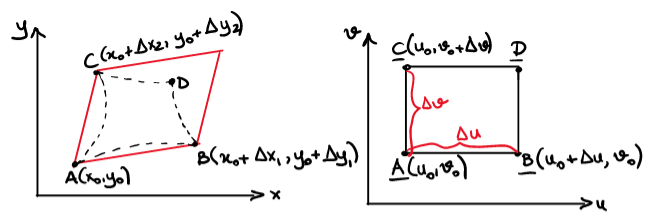
\includegraphics[width=\textwidth]{pic}
	\label{fig1}
\end{figure}

From Fig \ref{fig1}, we let
$$x = g(u,v)$$
and
$$y = h(u,v)$$
We have
$$\Delta x_1 = x_0 + x_1 - x_0 = g(u_0 + \Delta u, v_0) - g(u_0, v_0) = g_u(u_0,v_0)\Delta u$$
Similarly,
$$\Delta x_2 = g_v(u_0,v_0)\Delta v$$
$$\Delta y_1 = h_u(u_0,v_0)\Delta u$$
$$\Delta y_2 = h_v(u_0,v_0)\Delta v$$
The area in the $xy$ plane is then
\begin{align*}
||AB \times AC|| &= ||(\Delta x_1\hat{i} + \Delta y_1\hat{j}) \times (\Delta x_2\hat{i} + \Delta y_2\hat{j})|| \\
		 &= |\Delta x_1\Delta y_2 - \Delta x_2\Delta y_1| \\
		 &= |g_u\Delta uh_v\Delta v - g_v\Delta vh_u\Delta u| \\
		 &= \left| \text{det} \begin{bmatrix} g_u & g_v \\ h_u & h_v \end{bmatrix} \Delta u\Delta v \right| \\
\end{align*}

\begin{defn}
	We define the \textbf{Jacobian} as
	$$J = \left| \text{det} \begin{bmatrix} g_u & g_v \\ h_u & h_v \end{bmatrix} \right| = \left| \text{det} \begin{bmatrix} x_u & x_v \\ y_u & y_u \end{bmatrix} \right| = \frac{\partial(x,y)}{\partial(u,v)}$$
\end{defn}

We can then use the Jacobian to change the bases of integrals.
\end{document}
